\documentclass{standalone}
\usepackage{hsbcommon}
\begin{document}
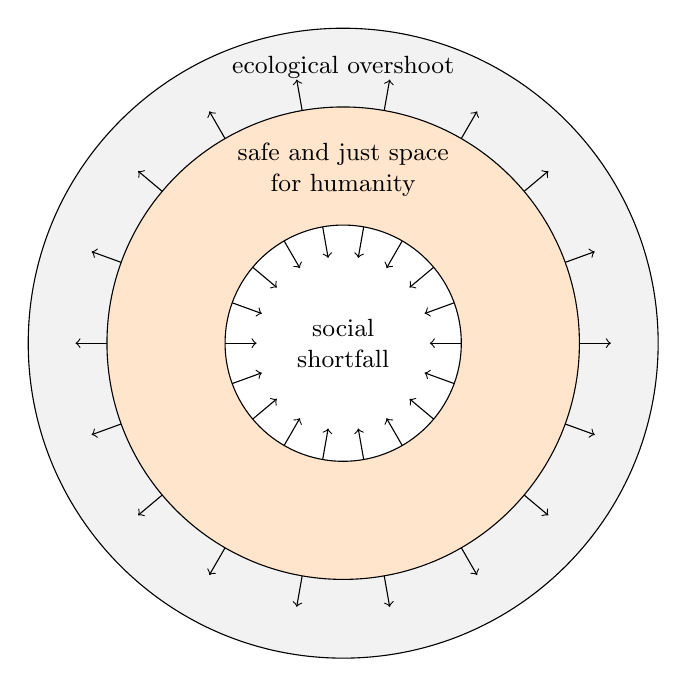
\begin{tikzpicture}
 
  % Radien (Gesamtdurchmesser = 8cm -> Außenradius = 4cm)
  \def\rOuter{4cm}   % Rand der ökologischen Überlastungszone
  \def\rMid{3cm}   % Außenrand des sicheren Raums (grüner Ring)
  \def\rInner{1.5cm} % Radius des Lochs (soziale Unterversorgung)
 
  % Ringe von außen nach innen zeichnen
  \draw[fill=gray!10] (0,0) circle (\rOuter);
  \draw[fill=orange!20] (0,0) circle (\rMid);
  \draw[fill=white] (0,0) circle (\rInner);

  \foreach \i in {0,20,...,350}
    {
    \draw[->] (\i:\rMid) -- (\i:\rMid+0.4cm);
    \draw[->] (\i:\rInner) -- (\i:\rInner-0.4cm);
    }
 
  % Beschriftung: sozialer Mangel (im Loch)
  \node[align=center, font=\small,text width=10ex] at (0,0) {social shortfall};
 
  % Beschriftung: sicherer Raum (im grünen Ring)
  \node[align=center, font=\small,text width=20ex] at (0,2.2cm) {safe and just space for humanity};
 
  % Beschriftung: ökologische Überlastung (außerhalb, mit Leader-Linie)
  % \draw (0,\rOuter) -- ++(1.2,0.8);
  \node[align=center, font=\small] at (0,3.5) {ecological overshoot};
 
\end{tikzpicture}

\end{document}